% Bachelor thesis defence slides
% Build: make   (uses latexmk -pdf)
\documentclass[aspectratio=169,11pt]{beamer}

% ----------------------------------------------------------------------------
% Theme
% ----------------------------------------------------------------------------
\usetheme{Copenhagen}
\usecolortheme{default}
\useinnertheme{rectangles}
\useoutertheme{miniframes}
\setbeamertemplate{navigation symbols}{}
\setbeamertemplate{footline}[frame number]
\usepackage{appendixnumberbeamer}
\usepackage{pgfpages}

% --- Speaker notes ---------------------------------------------------------
% Default: notes are stored in source but hidden from the projected PDF.
% To build a presenter-screen PDF (audience left, notes right) for pdfpc,
% comment out `hide notes' and uncomment `show notes on second screen=right'.
\setbeameroption{hide notes}
% \setbeameroption{show notes on second screen=right}

% ----------------------------------------------------------------------------
% Encoding, fonts, packages
% ----------------------------------------------------------------------------
\usepackage[T1]{fontenc}
\usepackage[utf8]{inputenc}
\usepackage{graphicx}
\usepackage{booktabs}
\usepackage{tabularx}
\usepackage{multirow}
\usepackage{xcolor}
\usepackage{amsmath, amssymb}
\usepackage{tikz}
\usetikzlibrary{positioning, arrows.meta, shapes.geometric, calc, backgrounds, fit}
\usepackage{tipa}            % phonetic eng (Ŋ/ŋ)
\usepackage{newunicodechar}

% Sami special characters (mirrored from thesis_report / iisa_paper)
\DeclareUnicodeCharacter{014A}{\raisebox{0.1ex}{\scalebox{1.3}{\textipa{\ng}}}}
\DeclareUnicodeCharacter{014B}{\textipa{\ng}}
\newcommand{\tstroke}{\mbox{\ooalign{t\cr\hspace{0.02em}\raisebox{0.49ex}{\rule{0.30em}{0.4pt}}}}}
\newcommand{\Tstroke}{\mbox{\ooalign{T\cr\hspace{0.04em}\raisebox{0.52ex}{\rule{0.52em}{0.45pt}}}}}
\DeclareUnicodeCharacter{0166}{\Tstroke}
\DeclareUnicodeCharacter{0167}{\tstroke}
\DeclareUnicodeCharacter{0110}{\DJ}
\DeclareUnicodeCharacter{0111}{\dj}

% Figure search paths so we can reuse thesis/IISA figures without copying
\graphicspath{%
  {./figures/}%
  {../thesis_report/summary_report/figures/}%
  {../iisa_paper/figures/}%
  {../../sami_ocr/test_data/account_of_sami/synthetic_images/}%
}

% SDU-ish accent (deep red) applied on top of Copenhagen's blue defaults
\definecolor{sduRed}{HTML}{B81818}
\definecolor{sduRedDark}{HTML}{8A1212}
\setbeamercolor{structure}{fg=sduRed}
\setbeamercolor{frametitle}{bg=sduRed, fg=white}
\setbeamercolor{title}{bg=sduRed, fg=white}
\setbeamercolor{section in head/foot}{bg=sduRedDark, fg=white}
\setbeamercolor{subsection in head/foot}{bg=sduRed, fg=white}
\setbeamercolor{alerted text}{fg=sduRed}
\setbeamercolor{block title}{bg=sduRed, fg=white}
\setbeamercolor{block body}{bg=sduRed!8}

% Smaller captions
\setbeamerfont{caption}{size=\scriptsize}

% ----------------------------------------------------------------------------
% Benchmark macros (kept in sync with thesis_report / iisa_paper)
% ----------------------------------------------------------------------------
\newcommand{\trocrBestCER}{8.55}
\newcommand{\trocrBestCharAcc}{91.45}
\newcommand{\trocrBestWordAcc}{71.84}
\newcommand{\trocrBestTime}{12.41}
\newcommand{\trocrSize}{350}
\newcommand{\ctcCER}{12.24}
\newcommand{\ctcWER}{37.35}
\newcommand{\ctcCharAcc}{87.76}
\newcommand{\ctcWordAcc}{62.65}
% Char/Word accuracies computed as 100 - CER and 100 - WER
\newcommand{\trocrSmiPredSynthCharAcc}{84.15}   % 100 - 15.85
\newcommand{\trocrSmiPredSynthWordAcc}{54.24}   % 100 - 45.76
\newcommand{\trocrSmiCharAcc}{75.88}            % 100 - 24.12
\newcommand{\trocrSmiWordAcc}{36.50}            % 100 - 63.50
\newcommand{\ctcTime}{0.033}
\newcommand{\ctcSize}{23}
\newcommand{\speedupFactor}{380}
\newcommand{\sizeRatio}{15}
\newcommand{\cerGap}{3.69}
\newcommand{\ctcThroughputK}{109}
\newcommand{\trocrThroughput}{290}
\newcommand{\millionPagesCtcHours}{10}
\newcommand{\millionPagesTrocrDays}{144}

\newcommand{\trocrSynthHFCER}{8.33}
\newcommand{\trocrSynthBookCER}{13.17}
\newcommand{\trocrSynthDeltaCER}{4.84}
\newcommand{\trocrSynthBookNormAcc}{45.8}
\newcommand{\ctcBookCER}{12.21}
\newcommand{\ctcBookNormAcc}{62.5}

\newcommand{\splitLongOriginalCER}{15.17}
\newcommand{\splitLongSplitCER}{8.12}
\newcommand{\splitShortCER}{12.04}
\newcommand{\splitImprovement}{7.05}
\newcommand{\splitPValue}{0.000009}
\newcommand{\splitCohensD}{1.35}
\newcommand{\splitImproveRate}{95}

\newcommand{\bleuScore}{10.40}
\newcommand{\chrfScore}{33.85}
\newcommand{\terScore}{76.30}

\newcommand{\trainSamples}{276{,}000}
\newcommand{\testSamples}{1{,}048}
\newcommand{\hfTestSamples}{1{,}000}
\newcommand{\bookTestSamples}{48}
\newcommand{\smiSpeakers}{25{,}000}
\newcommand{\turiYear}{1910}
\newcommand{\trocrInferenceIntroSec}{12}
\newcommand{\sentenceLengthThreshold}{80}

% ----------------------------------------------------------------------------
% Title block
% ----------------------------------------------------------------------------
\title{Optical Character Recognition\\of Low-Resource Languages}
\subtitle{Lightweight OCR for North S\'{a}mi Heritage Digitization}
\author{Jan Pawe\l{} Musio\l{}}
\institute{%
  Supervised by Aparna S. Varde \& Juan Heredia\\[0.3em]
  The Maersk Mc-Kinney M\o{}ller Institute\\
  University of Southern Denmark\\[0.5em]
  \scriptsize{\textit{Bachelor Thesis 2026~~\textbullet~~IISA 2026 full paper~~\textbullet~~SCAI 2026 abstract}}%
}
\date{June 2026}

\begin{document}

% ============================================================================
% Slide 1 - Title
% ============================================================================
\maketitle

% Table of contents
\begin{frame}{Outline}
  \tableofcontents[hideallsubsections]
\end{frame}

% ============================================================================
% PART 1 - FRAMING (~5 min)
% ============================================================================
\section{Motivation \& Research Question}

% ----------------------------------------------------------------------------
% Slide 2 - Why this matters
% ----------------------------------------------------------------------------
\begin{frame}{Why this matters}
  \begin{columns}[T,onlytextwidth]
    \column{0.46\textwidth}
    \begin{itemize}
      \item North S\'{a}mi is an indigenous Uralic language with $\sim$\smiSpeakers{} speakers in Northern Europe
      \item classified by UNESCO as \alert{definitely endangered}
      \item Heritage digitization is crucial for perserving the language and culture 
      \item My personal connection: low-resource Silesian language in southern Poland
    \end{itemize}
    \column{0.5\textwidth}
    \centering
    
\includegraphics[width=\linewidth]{sapmi1.jpg}\\[0.3em]
    \scriptsize\textit{S\'{a}pmi region across Norway, Sweden, Finland, Russia.}
  \end{columns}
\end{frame}
\note{%
\textbf{Open on the human stake, not on numbers.}

\textbf{Key facts to land:}
\begin{itemize}
  \item North S\'{a}mi: indigenous Uralic language, $\sim$25{,}000 speakers
  \item Nine mutually unintelligible S\'{a}mi varieties; some have $<$50 speakers (Pite, Ter, Ume \emph{critically endangered})
  \item UNESCO: \emph{definitely endangered} $-$ children no longer learn it as mother tongue at home
  \item S\'{a}pmi spans N.\ Norway, Sweden, Finland, Russia
\end{itemize}

\textbf{History one-liner:} centuries of suppression (Norwegianization, \emph{nomadskola}, boarding schools, Soviet collectivisation); Norway formally apologised in 2024 after the 2023 Truth \& Reconciliation report. The legacy is \emph{digital underrepresentation} $-$ a direct barrier to heritage digitisation.

\textbf{Personal:} mention Silesian briefly $-$ low-resource language from southern Poland, where I'm from. The democratisation-of-technology argument: same tools should be available to everyone, including endangered-language communities.

\textbf{Transition:} ``\dots this is where OCR comes in $-$ but the current OCR landscape has a problem.''
}

% ----------------------------------------------------------------------------
% Slide 3 - The gap
% ----------------------------------------------------------------------------
\begin{frame}{The gap}
  \begin{columns}[T,onlytextwidth]
    \column{0.42\textwidth}
    \textbf{State of the art:} TrOCR (National Library of Norway)
    \begin{itemize}
      \item \trocrBestCharAcc{}\% character accuracy
      \item \trocrSize{}~MB on disk
      \item \trocrInferenceIntroSec{}+ s / image on CPU
    \end{itemize}
    \medskip
    \alert{Not well fitted} for low-budget instituitons or individuals in low-resource settings such edge, mobile devices.
    \column{0.55\textwidth}
    \centering
    
\includegraphics[width=\linewidth]{design_space.pdf}\\[0.3em]
    \scriptsize\textit{Accuracy vs.\ size/latency.}
  \end{columns}
\end{frame}
\note{%
\textbf{The story:} SOTA exists, but cannot be deployed where it's needed most.

\textbf{SOTA = TrOCR variants from National Library of Norway}, released via Spr\r{a}kbanken, fine-tuned on synthetic S\'{a}mi data. Best variant (\texttt{trocr\_smi\_synth}):
\begin{itemize}
  \item $91.45$\% char.\ acc.\ ($8.55$\% CER)
  \item $\sim$350\,MB on disk
  \item $\sim$12.41\,s/image on CPU
  \item Throughput $\sim$290 images/hour
\end{itemize}

\textbf{Who's locked out?}
\begin{itemize}
  \item Community-driven preservation (small archives, museums)
  \item Mobile / field documentation in remote areas
  \item Institutions with no dedicated GPU budget
\end{itemize}

\textbf{Walk the design-space plot:} TrOCRs cluster in high-accuracy / high-size (lower-right). Classical OCR (Tesseract et al.) is cheap but bad on S\'{a}mi ($>$30\% CER per Enstad et al.\ 2025). \alert{The upper-left target zone $-$ accurate and small $-$ is empty.}

\textbf{One more weight:} Enstad et al.\ note that current OCR accuracy ``remains insufficient for downstream NLP tasks'' $-$ so both accuracy \emph{and} deployability are problems worth solving.

\textbf{Transition:} ``\dots which leads to the research question.''
}

% ----------------------------------------------------------------------------
% Slide 4 - Research question + contributions
% ----------------------------------------------------------------------------
\begin{frame}{Research question \& contributions}
  \begin{block}{Research question}
    \textit{Can a lightweight OCR architecture approach Transformer-level accuracy
    for North S\'{a}mi while enabling practical deployment on modest hardware?}
  \end{block}
  \medskip
  \footnotesize
  \textbf{Six contributions (listed in IISA paper):}
  \begin{enumerate}
    \item Lightweight CNN-CTC architecture for North S\'{a}mi OCR
    \item Systematic benchmark vs.\ 7 TrOCR + 3 pretrained-CTC variants
    \item Sustainable-AI footprint: \speedupFactor{}$\times$ faster, \sizeRatio{}$\times$ smaller
    \item Conjunction-based sentence splitting (proof of concept)
    \item End-to-end OCR$\rightarrow$MT pipeline with TartuNLP
    \item Applications in 21st-century education, NLP \& robotics
  \end{enumerate}
\end{frame}
\note{%
\textbf{Read the question verbatim, slowly:}\\
\emph{``Can a lightweight OCR architecture approach Transformer-level accuracy for North S\'{a}mi while enabling practical deployment on modest hardware?''}

\textbf{Why this phrasing matters:} the question is \emph{two-headed}. Accuracy \emph{and} deployability. Most OCR research optimises only the first; this thesis treats the second as a first-class constraint.

\textbf{Six contributions $-$ name each in one breath, not in detail:}
\begin{enumerate}
  \item Lightweight CNN-CTC architecture (the \texttt{ctc\_simple} model)
  \item Systematic benchmark: ours vs.\ 7 TrOCR variants + 3 pretrained-CTC variants
  \item Sustainable-AI footprint argument (380$\times$ faster, 15$\times$ smaller)
  \item Conjunction-based sentence splitting (linguistically motivated preprocessing)
  \item End-to-end OCR$\rightarrow$MT pipeline with TartuNLP API
  \item Applications: 21st-century education, NLP, next-gen robotics
\end{enumerate}

\textbf{Frame as a map:} ``Each of these will reappear later in the talk $-$ this slide is the table of contents for the rest.''

\textbf{Transition:} ``\dots before showing the results I need to give just enough background on what makes North S\'{a}mi hard for OCR.''
}

% ============================================================================
% PART 2 - BACKGROUND (~3 min)
% ============================================================================
\section{Background}

% ----------------------------------------------------------------------------
% Slide 5 - What makes North Sami hard for OCR
% ----------------------------------------------------------------------------
\begin{frame}{What makes North S\'{a}mi hard for OCR}
  \begin{columns}[T,onlytextwidth]
    \column{0.46\textwidth}
    \footnotesize
    \begin{enumerate}
      \item \textbf{Seven special diacritics}\\
        \'{a}, \v{c}, đ, ŋ, \v{s}, ŧ, \v{z}
      \item \textbf{Agglutinative morphology}\\
        Hundreds of inflected forms per verb, large type-token ratio $\rightarrow$
        model cannot memorise word shapes.
      \item \textbf{Consonant gradation}\\
        \textit{giella} (``language'') vs.\ \textit{giela} (``of language'') $-$
        a single dropped ``\textit{l}'' changes the meaning.
    \end{enumerate}
    \medskip
    \column{0.5\textwidth}
    \centering
    
\includegraphics[width=\linewidth]{combined_example.pdf}\\[0.3em]
    \scriptsize\textit{Seven characters foreign to standard Latin script.}
  \end{columns}
\end{frame}
\note{%
\textbf{Three pillars. This slide double-duties as the ``why character accuracy matters'' setup.}

\textbf{1. Seven special diacritics:} \'{a}, \v{c}, đ, ŋ, \v{s}, ŧ, \v{z} (and capitals).
\begin{itemize}
  \item Several visually very close to plain Latin: \v{c}/c, \v{s}/s, \v{z}/z, ŧ/t
  \item đ and ŧ have \emph{no} visual analog in major European languages
  \item Reliable recognition of these is one of the central technical challenges
\end{itemize}

\textbf{2. Agglutinative morphology.}
\begin{itemize}
  \item Hundreds of inflected forms per verb; six cases in singular/plural, plus dual for pronouns/verbs
  \item Words built by stacking morphemes: \emph{viesuiguin} = ``with the houses'' = viesu (house) + i (plural) + guin (comitative)
  \item $\Rightarrow$ huge type-token ratio: model rarely sees same word twice; must learn the script at character level
\end{itemize}

\textbf{3. Consonant gradation.}
\begin{itemize}
  \item \emph{giella} ``language'' (double l) vs.\ \emph{giela} ``of language'' (single l)
  \item A single dropped character flips the grammatical role
  \item Also a three-way quantity contrast (short / long / overlong); only partly captured in spelling
\end{itemize}

\textbf{Orthographic note:} unified S\'{a}mi orthography only adopted 1979 (revised 1985). Turi's 1910 book uses Friis orthography $-$ relevant for the OOD set later.

\textbf{Land the takeaway:} ``\dots so when we look at OCR error rates later, remember a single-character error in S\'{a}mi can change \emph{grammatical meaning}, not just produce a typo.''
}

% ----------------------------------------------------------------------------
% Slide 6 - CNN-CTC vs TrOCR in one picture
% ----------------------------------------------------------------------------
\begin{frame}{Two architectural families}
  \begin{columns}[T,onlytextwidth]
    \column{0.48\textwidth}
    \textbf{CNN-CTC} (CRNN family)
    \begin{itemize}
      \item CNN $\rightarrow$ column features
      \item Reads image left to right
      \item No alignment supervision needed
      \item Small, fast
    \end{itemize}
    \column{0.48\textwidth}
    \textbf{TrOCR} (Transformer)
    \begin{itemize}
      \item ViT encoder $+$ autoregressive decoder
      \item Image patches $\rightarrow$ self-attention
      \item Token-by-token generation
      \item Large, accurate, slow
    \end{itemize}
  \end{columns}
  \vspace{1em}
  \centering
  \footnotesize\textit{Same task, very different inductive biases and deployment profiles.}
\end{frame}
\note{%
\textbf{Keep this conceptual; details live in the thesis appendix if asked.}

\textbf{CRNN family (Shi et al.\ 2017, what we use):}
\begin{itemize}
  \item CNN extracts spatial features $\rightarrow$ adaptive pool to height 1 $\rightarrow$ a sequence of \emph{column vectors} running left to right
  \item Optional sequence encoder (BiLSTM or Transformer) adds temporal context
  \item CTC head + loss: \emph{no character-level segmentation needed}. CTC marginalises over all alignments via a blank token
  \item End-to-end trainable, small, fast, explainable
\end{itemize}

\textbf{TrOCR (Li et al.\ 2023):}
\begin{itemize}
  \item Vision Transformer encoder: image split into fixed-size \emph{patches}, processed with self-attention
  \item Autoregressive decoder (GPT-2-style): generates text \emph{token by token}, conditioned on encoded image and previous outputs
  \item Pre-trained on massive image corpora, then fine-tuned $-$ uses transfer at scale
  \item Higher accuracy, but compute/memory cost is much larger
\end{itemize}

\textbf{Land:} ``Same task, very different inductive biases. CRNN treats the line as a 1D sequence by construction; TrOCR treats it as a 2D image and a language-modelling problem. The cost difference follows from that.''
}

% ============================================================================
% PART 3 - WHAT WAS BUILT (~4 min)
% ============================================================================
\section{What was built}

% ----------------------------------------------------------------------------
% Slide 7 - Modular pipeline
% ----------------------------------------------------------------------------
\begin{frame}{A modular OCR pipeline}
  \begin{columns}[T,onlytextwidth]
    \column{0.50\textwidth}
    \textbf{Design space:} 5 backbones $\times$ 3 encoders, shared CTC head
    \begin{itemize}
      \item Backbones: SimpleCNN, VGG16/19, ResNet50/101
      \item Encoders: none, BiLSTM, Transformer
      \item $\rightarrow$ 15 configurations
    \end{itemize}
    \medskip
    \footnotesize
    \alert{Trained only 4} due to compute budget (V100, single GPU).\\
    Architecture deliberately extensible, not incomplete.
    \column{0.48\textwidth}
    \centering
    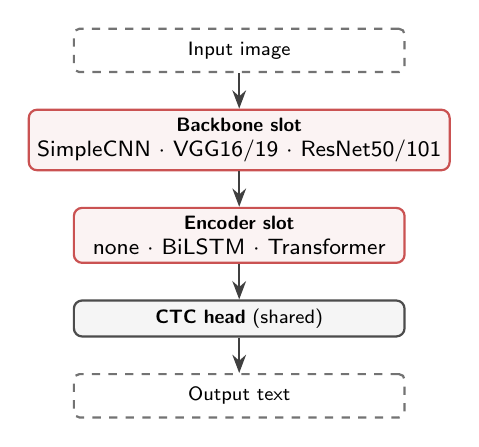
\begin{tikzpicture}[
        font=\scriptsize\sffamily,
        >=Stealth,
        node distance=0.45cm,
        io/.style={draw=black!55, thick, dashed, rounded corners=2pt,
                   minimum width=4.2cm, minimum height=0.55cm, align=center},
        slot/.style={draw=sduRed!75, thick, rounded corners=3pt,
                     minimum width=4.2cm, align=center, fill=sduRed!5,
                     inner sep=3pt},
        fixed/.style={draw=black!70, thick, rounded corners=3pt,
                      minimum width=4.2cm, align=center, fill=gray!8,
                      inner sep=3pt},
        arrow/.style={->, thick, draw=black!75},
      ]
      \node[io] (input) {Input image};
      \node[slot, below=of input] (bb) {%
        \textbf{Backbone slot}\\[1pt]
        \footnotesize SimpleCNN $\cdot$ VGG16/19 $\cdot$ ResNet50/101%
      };
      \node[slot, below=of bb] (enc) {%
        \textbf{Encoder slot}\\[1pt]
        \footnotesize none $\cdot$ BiLSTM $\cdot$ Transformer%
      };
      \node[fixed, below=of enc] (ctc) {%
        \textbf{CTC head} (shared)%
      };
      \node[io, below=of ctc] (out) {Output text};
      \draw[arrow] (input) -- (bb);
      \draw[arrow] (bb)    -- (enc);
      \draw[arrow] (enc)   -- (ctc);
      \draw[arrow] (ctc)   -- (out);
    \end{tikzpicture}\\[0.2em]
    \scriptsize\textit{Three swappable slots, queue training.}
  \end{columns}
\end{frame}
\note{%
\textbf{Slot-based design $-$ explain why this matters.}

\textbf{Three swappable slots:} backbone (feature extraction) $\rightarrow$ encoder (sequence context) $\rightarrow$ CTC head (transcription).
\begin{itemize}
  \item Backbones: SimpleCNN, VGG16, VGG19, ResNet50, ResNet101
  \item Encoders: none, BiLSTM (2 layers), Transformer encoder block
  \item Decoder fixed (CTC) across all variants $\Rightarrow$ accuracy differences attribute to the swapped slot
  \item $5 \times 3 = 15$ configurations on paper
\end{itemize}

\textbf{Compute reality:}
\begin{itemize}
  \item V100 32GB on uCloud (SDU/DeiC), single GPU
  \item Per-epoch time: $\sim$8 min (SimpleCNN), $\sim$19 min (VGG pair), $\sim$76 min (ResNet50)
  \item Full 100-epoch ResNet50 would have been $\sim$5 days $\rightarrow$ ResNet101 gated on the ResNet50 result and not trained
  \item Trained 4 variants total: \texttt{ctc\_simple} (full 100 ep), \texttt{ctc\_vgg16} (stopped 52 ep), \texttt{ctc\_vgg19} (63 ep), \texttt{ctc\_resnet50} (37 ep $\sim$ 48\,h)
\end{itemize}

\textbf{Frame deliberately:} ``This is a scoped study within an extensible framework, not an incomplete one. The harness already supports adding new models $-$ adding Tesseract or trying ResNet101 with more compute is a follow-on, not a re-design.''

\textbf{Transition:} ``\dots and the headline variant is the simplest one in the design space.''
}

% ----------------------------------------------------------------------------
% Slide 8 - The headline model
% ----------------------------------------------------------------------------
\begin{frame}{The headline model: CNN-CTC (\texttt{ctc\_simple})}
  \begin{columns}[T,onlytextwidth]
    \column{0.55\textwidth}
    \begin{itemize}
      \item \textbf{7-layer SimpleCNN} trained from scratch
      \item \textbf{No encoder} (direct CNN $\rightarrow$ CTC)
      \item \textbf{$\sim$6M params, \ctcSize{}~MB on disk}
    \end{itemize}
    \medskip
    \textbf{Asymmetric pooling to reduce height while preserving horizontal resolution}
    \begin{itemize}
      \item $2\times2$ early layers (collapse both axes)
      \item $2\times1$ later layers (preserve horizontal resolution)
      \item Adaptive pool to height 1 $\rightarrow$ column sequence
    \end{itemize}
    \medskip
    \footnotesize\textit{Preserves character ordering that CTC depends on.}
    \column{0.42\textwidth}
    \centering
    
\includegraphics[width=\linewidth,height=0.75\textheight,keepaspectratio]{architecture_tikz.pdf}
  \end{columns}
\end{frame}
\note{%
\textbf{Walk the architecture, but do not lecture on layer widths.}

\textbf{Architecture spec}
\begin{itemize}
  \item 7-layer SimpleCNN, channels $64{\to}128{\to}256{\to}256{\to}512{\to}512{\to}512$, each followed by BN $+$ ReLU
  \item Trained from scratch (no ImageNet weights) on Spr\r{a}kbanken
  \item No encoder slot $\rightarrow$ direct CNN $\rightarrow$ CTC
  \item $\sim$6M parameters, \ctcSize\,MB on disk
\end{itemize}

\textbf{Asymmetric pooling $-$ the key trick:}
\begin{itemize}
  \item Early layers: $2\times2$ max pooling (collapse both axes)
  \item Later layers: $2\times1$ pooling (collapse only height, preserve horizontal resolution)
  \item Final adaptive pool collapses height to 1 $\rightarrow$ sequence of column vectors
\end{itemize}

\textbf{Why this matters:} CTC reads the output left to right and aligns columns to characters. If horizontal resolution dies in the backbone, character ordering dies with it. Asymmetric pooling preserves exactly the dimension CTC needs.

\textbf{Tail of the pipeline:} column vectors projected $512 \rightarrow 256$, linear head to $395$ classes ($394$ chars + CTC blank), LogSoftmax, greedy decoding at inference.

\textbf{Training:} CTC loss, AdamW lr $10^{-4}$, weight decay $10^{-4}$, batch 32, gradient clip 5.0, 100 epochs at $\sim$8 min/epoch $=$ $\sim$13 hours on V100.

\textbf{Land:} ``\dots smallest meaningful baseline in the design space, and the one we get the most out of.''
}

% ----------------------------------------------------------------------------
% Slide 9 - Setup
% ----------------------------------------------------------------------------
\begin{frame}{Experimental setup}
  \footnotesize
  \begin{description}
    \item[Train] Spr\r{a}kbanken synthetic S\'{a}mi OCR dataset (National Library of Norway), $\sim$307k line images (276k training + 31k hyperparameter tuning), 32$\times$800px.  
    \item[Test] \testSamples{} samples
      \begin{itemize}
        \item \hfTestSamples{} in-domain synthetic lines (Spr\r{a}kbanken validation split)
        \item \bookTestSamples{} out-of-domain parallel Northern S\'{a}mi--English sentences from Turi's 1910 "An Account of S\'{a}mi"
      \end{itemize}
    \item[Metrics] CER, WER, exact match, normalised accuracy (raw UTF-8)
    \item[Hardware] Nvidia V100 32GB for training and \alert{CPU-only inference benchmark}
      to simulate resource-constrained deployment. 
  \end{description}
  \medskip
  \centering
\end{frame}
\note{%
\textbf{Brief slide. The point is to establish that the comparison is fair.}

\textbf{Train data $-$ Spr\r{a}kbanken (NLN)}
\begin{itemize}
  \item Synthetic North S\'{a}mi OCR corpus, line-level
  \item $307{,}387$ training samples $\rightarrow$ $276{,}000$ (90\%) used for training, $\sim$31{,}000 (10\%) for hyperparameter tuning / early stopping
  \item 32$\times$800 px, varied fonts/spacing/noise/background to simulate scanned text
  \item Charset: $394$ unique characters $+$ 1 CTC blank $=$ $395$ classes
\end{itemize}

\textbf{Test data $-$ \testSamples{} samples}
\begin{itemize}
  \item \hfTestSamples{} in-domain from Spr\r{a}kbanken \emph{validation} split (held out, never seen during training)
  \item \bookTestSamples{} out-of-domain $-$ hand-picked sentences from Turi's $\turiYear{}$ \emph{Muitalus s\'{a}miid birra}, synthetically rendered
  \item Important: OOD set tests \emph{lexical/morphological} generalization, not scan-quality robustness
\end{itemize}

\textbf{Metrics:} CER (char-level Levenshtein), WER (word-level), exact-match accuracy, normalised accuracy (after stripping punctuation and collapsing whitespace). All raw UTF-8, no NFC/NFKC normalization.

\textbf{Hardware framing $-$ pre-empt a question:}
\begin{itemize}
  \item Training on NVIDIA V100 32GB (uCloud, SDU/DeiC)
  \item Inference benchmark on \emph{AMD Ryzen 5 PRO laptop CPU} $-$ deliberately a realistic deployment target, not ideal serving hardware
\end{itemize}

\textbf{Fair-comparison note:} TrOCR variants used as released by NLN without additional fine-tuning $-$ a baseline-as-shipped comparison.
}

% ============================================================================
% PART 4 - RESULTS (~6 min, the heart of the talk)
% ============================================================================
\section{Results}

% ----------------------------------------------------------------------------
% Slide 10 - Main benchmark
% ----------------------------------------------------------------------------
\begin{frame}{Main benchmark}
  \footnotesize
  \begin{table}
    \centering
    \begin{tabular}{@{}lrrrr@{}}
      \toprule
      \textbf{Model} & \textbf{Char.\ Acc.\ \%}~$\uparrow$ & \textbf{Word Acc.\ \%}~$\uparrow$ & \textbf{sec / img} & \textbf{Size (MB)} \\
      \midrule
      trocr\_smi\_synth        & \textbf{\trocrBestCharAcc}      & \textbf{\trocrBestWordAcc}      & \trocrBestTime         & $\sim$\trocrSize \\
      \textbf{ctc\_simple}     & \ctcCharAcc                      & \ctcWordAcc                      & \textbf{\ctcTime}      & \textbf{\ctcSize} \\
      trocr\_smi\_pred\_synth  & \trocrSmiPredSynthCharAcc        & \trocrSmiPredSynthWordAcc        & 12.08                  & $\sim$\trocrSize \\
      trocr\_smi               & \trocrSmiCharAcc                 & \trocrSmiWordAcc                 & 16.23                  & $\sim$\trocrSize \\
      \bottomrule
    \end{tabular}\\[2pt]
    \scriptsize\textit{Char.\ Acc.\ $= 100 - \textrm{CER}$\quad Word Acc.\ $= 100 - \textrm{WER}$}
  \end{table}
  \medskip
  \textbf{Results for \texttt{ctc\_simple}:}\\[0.3em]
  \alert{\ctcCharAcc{}\% char.\ acc.\ (within \cerGap{}\,pp of best TrOCR), \speedupFactor{}$\times$ faster, \sizeRatio{}$\times$ smaller.}\\[0.6em]
  \footnotesize
  Consequently: 1\,M-page corpus takes \alert{$<$\millionPagesCtcHours{} hours} on CPU
  vs.\ $\sim$\millionPagesTrocrDays{} days for TrOCR.
\end{frame}
\note{%
\textbf{Heart of the talk. Slow down here.}

\textbf{Land one number, repeat it:}
\begin{itemize}
  \item \texttt{ctc\_simple} $=$ \ctcCharAcc{}\% char.\ acc.\ ($=100-$CER), \ctcWordAcc{}\% word acc.
  \item Best TrOCR $=$ \trocrBestCharAcc{}\% char.\ acc., \trocrBestWordAcc{}\% word acc.
  \item \textbf{Gap: \cerGap{} pp on CER} (i.e., the headline accuracy comparison)
\end{itemize}

\textbf{Now flip to efficiency:}
\begin{itemize}
  \item \speedupFactor{}$\times$ faster on the same CPU
  \item \sizeRatio{}$\times$ smaller (\ctcSize\,MB vs \trocrSize\,MB)
  \item Throughput: $\sim$109{,}000 img/hour vs $\sim$290 img/hour for TrOCR
\end{itemize}

\textbf{Translate to something tangible $-$ this is the line the committee will remember:}
\begin{itemize}
  \item A 1\,M-page corpus processable in $<$\millionPagesCtcHours\,hours on a CPU vs.\ $\sim$\millionPagesTrocrDays\,days for TrOCR
  \item Edge-deployable (fits on a phone) vs.\ requires a server
\end{itemize}

\textbf{Quick context on the other rows:}
\begin{itemize}
  \item Other TrOCR variants degrade quickly without synthetic pretraining (\texttt{trocr\_smi} alone: $75.88$\% char acc)
  \item \texttt{ctc\_simple} sits between the best and second-best TrOCR variant despite being $15\times$ smaller
\end{itemize}

\textbf{Definition note:} char.\ acc.\ here is $100-$CER. Strictly speaking CER counts insertions too, so directly measured char.\ acc.\ is slightly different ($\sim$91.56\% vs $91.45\%$) $-$ I report the simpler $100-$CER definition consistently.
}

% ----------------------------------------------------------------------------
% Slide 11 - The surprising finding (OOD)
% ----------------------------------------------------------------------------
\begin{frame}{Out-of-domain evaluation gave a surprising finding}
  \begin{columns}[T,onlytextwidth]
    \column{0.48\textwidth}
    \footnotesize
    On Turi's \turiYear{} historical text:
    \begin{itemize}
      \item TrOCR degrades \trocrSynthDeltaCER{}\,pp
        (\trocrSynthHFCER{}\% $\rightarrow$ \trocrSynthBookCER{}\%)
      \item \texttt{ctc\_simple} stays flat
        (\ctcCER{}\% $\rightarrow$ \ctcBookCER{}\%)
      \item Normalised accuracy: \alert{\ctcBookNormAcc{}\% vs.\ \trocrSynthBookNormAcc{}\%}
    \end{itemize}
    \medskip
    \textbf{But!}\\
    $n = \bookTestSamples{}$ samples.
    \alert{Not conclusive, might suggest...}\\
    The CNN-CTC is more stable but results lack statistical power. 
    \column{0.5\textwidth}
    \centering
    
\includegraphics[width=\linewidth]{per_dataset_comparison.png}
  \end{columns}
\end{frame}
\note{%
\textbf{Surface the finding slowly $-$ this is the one ``unexpected'' result.}

\textbf{In-domain numbers (Spr\r{a}kbanken val):}
\begin{itemize}
  \item TrOCR (\texttt{trocr\_smi\_synth}): $8.33$\% CER
  \item \texttt{ctc\_simple}: $12.24$\% CER
\end{itemize}

\textbf{Out-of-domain (Turi 1910 historical text, Friis orthography):}
\begin{itemize}
  \item TrOCR: $13.17$\% CER $\rightarrow$ degrades by \trocrSynthDeltaCER\,pp
  \item \texttt{ctc\_simple}: $12.21$\% CER $\rightarrow$ essentially flat ($-0.03$\,pp)
  \item One TrOCR variant (\texttt{trocr\_smi\_pred\_synth}) still beats us on raw book CER ($11.00$\%)
\end{itemize}

\textbf{The headline though:} after punctuation+whitespace normalisation, \texttt{ctc\_simple} \emph{overtakes all TrOCRs}: \ctcBookNormAcc\% vs \trocrSynthBookNormAcc\% / $43.8$\%.

\textbf{Hypothesis (state cautiously):} smaller model learns more transferable character-level features and is less prone to overfitting synthetic rendering artefacts. Consistent with Enstad et al.\ noting that the ``pred'' (auto-transcribed) variant helps with domain shift.

\textbf{PRE-EMPT THE CRITIQUE BEFORE THEY DO:}
\begin{itemize}
  \item $n=$\bookTestSamples{}, single 1910 book, low statistical power
  \item Phrase as ``suggestive, not conclusive''
  \item Strength: \emph{consistent across multiple metrics} (CER, normalised acc., variant ranking) rather than statistically powered
\end{itemize}

\textbf{Important caveat:} this tests \emph{lexical / orthographic} generalization (vocabulary and spelling), \emph{not} scan-quality robustness $-$ images are synthetically rendered. Real-scan validation is open future work.
}

% ----------------------------------------------------------------------------
% Slide 12 - Conjunction splitting
% ----------------------------------------------------------------------------
\begin{frame}{Conjunction-based sentence splitting}
  \begin{columns}[T,onlytextwidth]
    \column{0.5\textwidth}
    \footnotesize
    Long sentences are over the fixed 800\,px input width.\\[0.3em]
    Split at North S\'{a}mi conjunctions
    (\textit{ja}, \textit{muhto}, \textit{dahje}, \textit{go}, \textit{ahte}, \textit{jos}),
    OCR each segment, rejoin.
    \medskip
    \begin{itemize}
      \item Long-sentence CER:
        \alert{\splitLongOriginalCER{}\% $\rightarrow$ \splitLongSplitCER{}\%}
        ($-$\splitImprovement{}\,pp)
      \item Below short-sentence baseline (\splitShortCER{}\%)
      \item $p = \splitPValue{}$, Cohen's $d = \splitCohensD{}$
      \item \splitImproveRate{}\% of split samples improved, none degraded
    \end{itemize}
    \medskip
    \alert{Oracle upper bound:} splitting operates on ground-truth strings, the cut images are re-rendered without noise.
    After deployment, much of the gain would be lost. 
    \column{0.48\textwidth}
    \centering
    
\includegraphics[width=\linewidth]{split_comparison.pdf}
  \end{columns}
\end{frame}
\note{%
\textbf{Most likely slide to draw a hard question. Owning the caveat first is essential.}

\textbf{Motivation:} per-sentence error analysis showed a steep accuracy drop beyond $\sim$80 characters $-$ the fixed 800\,px input width compresses longer sentences. The conjunction \emph{ja} (``and'') dominates the word distribution, which suggested splitting at conjunction boundaries.

\textbf{What gets split on:}
\begin{itemize}
  \item Coordinate conjunctions: \emph{ja}, \emph{muhto} (but), \emph{dahje} (or)
  \item Subordinate conjunctions: \emph{go} (when/because), \emph{ahte} (that), \emph{jos} (if)
  \item Multi-word forms greedily first: \emph{ovdal go} (before), \emph{dasgo} (because)
\end{itemize}

\textbf{Mechanics:} regex on word boundaries (case-insensitive). Split immediately \emph{before} a conjunction (it stays with the following clause). Minimum segment length 20 chars to avoid over-splitting when conjunctions cluster. Each segment re-rendered as fresh synthetic image, OCR independently, rejoined with single spaces.

\textbf{Numbers, crisp:}
\begin{itemize}
  \item Long-sentence CER: $15.17$\% $\rightarrow$ $8.12$\% ($-7.05$\,pp)
  \item Now \emph{below} the short-sentence baseline ($12.04$\%) $-$ length penalty eliminated
  \item Paired test $p = 0.000009$, Cohen's $d = 1.35$ (very large effect)
  \item 95\% of split samples improved, none degraded
\end{itemize}

\textbf{The caveat $-$ say it before they ask:}
\begin{itemize}
  \item Splitter operates on \emph{ground truth} strings, not noisy OCR predictions
  \item Each segment re-rendered as a \emph{fresh clean} synthetic image
  \item So this is an \emph{oracle upper bound}, on both segmentation and image quality
  \item Real deployment would have to detect conjunctions on noisy OCR (short tokens like \emph{ja}, \emph{go} are themselves error-prone) or fall back to whitespace-based segmentation $-$ likely loses much of the $7.05$\,pp
\end{itemize}

\textbf{Frame:} ``proof of concept showing that linguistically motivated preprocessing can mitigate the length penalty without architectural changes. Productionizing it is open work.''
}

% ----------------------------------------------------------------------------
% Slide 13 - End-to-end OCR -> MT
% ----------------------------------------------------------------------------
\begin{frame}{End-to-end OCR\,$\rightarrow$\,MT pipeline}
  \footnotesize
  Predicted text from \texttt{ctc\_simple} fed to TartuNLP's North~S\'{a}mi\,$\rightarrow$\,English API.
  \smallskip
  \begin{columns}[T,onlytextwidth]
    \column{0.34\textwidth}
    \centering
    \begin{tabular}{lc}
      \toprule
      \textbf{Metric} & \textbf{Score} \\
      \midrule
      BLEU & \bleuScore{} \\
      chrF & \chrfScore{} \\
      TER  & \terScore{}\% \\
      \bottomrule
    \end{tabular}
    \medskip\\
    {\raggedright
    \textbf{Why moderate?} Character errors land on \alert{morphological suffixes} that carry grammatical role $-$ a single dropped character flips the meaning of a whole clause.\\[0.4em]
    Good for \emph{indexing / content discovery}, not full translation.\par}

    \column{0.62\textwidth}
    \textbf{Example (entry 998, CER 1.2\%):}\\[2pt]
    \includegraphics[width=\linewidth]{entry_998.png}\\[2pt]
    \scriptsize
    \textbf{GT (s\'{a}mi):} \emph{ja \'{a}ldoeallu lea v\'{a}rala\v{s} dan galggalii s\'{a}httit nu \alert{siivvut} reainnidit go lea m\'{a}ŧola\v{s}}\\[1pt]
    \textbf{Pred (s\'{a}mi):} \emph{\dots s\'{a}httit nu \alert{siivut} reainnidit \dots}\hfill\textit{[one ``v'' dropped]}\\[6pt]
    \textbf{GT (en):} ``and it is a \alert{dangerous time for the cow herd}, they must be \alert{herded} as carefully as possible.''\\[2pt]
    \textbf{Pred (en):} ``and \alert{the livestock is dangerous}, it should be able to be \alert{removed} as safely as possible.''
  \end{columns}
\end{frame}
\note{%
\textbf{The score is moderate $-$ the interesting part is \emph{why}.}

\textbf{Setup:}
\begin{itemize}
  \item Predicted text from \texttt{ctc\_simple} (at $12.24$\% CER) fed to TartuNLP's North~S\'{a}mi$\rightarrow$English neural MT API
  \item Scored against English reference on the OOD parallel set (Turi 1910)
\end{itemize}

\textbf{Scores:}
\begin{itemize}
  \item BLEU $10.40$ (n-gram precision, brutal on morphological variation)
  \item chrF $33.85$ (character-level F-score $-$ more forgiving of morphology, still moderate)
  \item TER $76.30$\% (translation edit rate; closer to 0 is better)
\end{itemize}

\textbf{Why ``moderate'' \emph{makes sense} here $-$ explain the causal chain:}
\begin{itemize}
  \item At $12.24$\% CER, most character errors land on the word \emph{endings}
  \item North S\'{a}mi is agglutinative: suffixes encode case, number, possession, tense
  \item A single dropped character can flip the grammatical role of a whole clause
  \item OCR errors therefore propagate \emph{disproportionately} into MT errors
\end{itemize}

\textbf{Frame the pipeline honestly:}
\begin{itemize}
  \item Viable for archival indexing and content discovery
  \item Not (yet) for fluent automatic translation
  \item This also underscores the need for open-access MT bridges to low-resource languages
\end{itemize}

\textbf{Walk the example (entry 998) $-$ the cleanest case in the test set:}
\begin{itemize}
  \item OCR is almost perfect: CER 1.2\%, \emph{one} character difference $-$ \emph{siivvut} $\rightarrow$ \emph{siivut} (one ``v'' dropped)
  \item That single character is a verbal inflection marker
  \item Effects on the MT output cascade:
    \begin{itemize}\scriptsize
      \item Subject of ``dangerous'' flips: ``\alert{a dangerous time} for the cow herd'' $\rightarrow$ ``\alert{the livestock} is dangerous''
      \item Verb meaning flips: ``\alert{herded} as carefully as possible'' $\rightarrow$ ``\alert{removed} as safely as possible''
    \end{itemize}
  \item One-line takeaway: \alert{one character $\rightarrow$ wrong subject, wrong verb, wrong meaning}
  \item Memorable point: the MT does \emph{not} flag uncertainty; the cascade silently produces fluent but unrelated English
\end{itemize}

\textbf{Transition:} ``\dots one more result is worth showing $-$ a negative one.''
}

% ----------------------------------------------------------------------------
% Slide 14 - Negative result
% ----------------------------------------------------------------------------
\begin{frame}{Negative result: ImageNet pretraining failed}
  \begin{columns}[T,onlytextwidth]
    \column{0.46\textwidth}
    \footnotesize
    Three pretrained backbones $-$ VGG16, VGG19, ResNet50 $-$ \alert{all $>$69\% CER}.
    \medskip
    \begin{itemize}
      \item VGG pair: \emph{underfits} (train loss barely moves)
      \item ResNet50: \emph{overfits} (train collapses, val stuck)
      \item Same head and projection layer as \texttt{ctc\_simple}
    \end{itemize}
    \medskip
    \textbf{Hypothesis:} ImageNet's object-level features misalign with
    character-stroke topology.\\[0.3em]
    \emph{Couldn't try again due to compute budget.}
    \column{0.52\textwidth}
    \centering
    
\includegraphics[width=\linewidth]{training_curves.pdf}
  \end{columns}
  \medskip
  \centering
\end{frame}
\note{%
\textbf{Frame a negative result as scientific maturity, not a footnote.}

\textbf{Setup:} three CTC variants with ImageNet-pretrained backbones (\texttt{ctc\_vgg16}, \texttt{ctc\_vgg19}, \texttt{ctc\_resnet50}), \emph{same} projection layer and CTC head as \texttt{ctc\_simple}. Only the backbone differs.

\textbf{All three failed:}
\begin{itemize}
  \item \texttt{ctc\_vgg16}: $73.94$\% CER, $0$\% exact match
  \item \texttt{ctc\_vgg19}: $71.86$\% CER, $0$\% exact match
  \item \texttt{ctc\_resnet50}: $75.30$\% CER, $0$\% exact match
\end{itemize}

\textbf{Two distinct signatures (point to plot):}
\begin{itemize}
  \item VGG pair: \emph{underfits}. Training loss $0.81 \rightarrow 0.60$ over $\sim$60 epochs; validation CER never breaks $0.72$
  \item ResNet50: \emph{overfits}. Train loss $0.80 \rightarrow 0.23$ in 37 epochs; val CER flat at $0.73$; val loss bounces upward
\end{itemize}

\textbf{Rules out simple causes:}
\begin{itemize}
  \item \texttt{ReduceLROnPlateau} repeatedly halved the LR with no effect $-$ not an LR or gradient-instability problem
  \item Effective LR on pretrained backbone was already very low ($3\times 10^{-5}$ base $\times$ $0.1$ differential $=$ $3\times 10^{-6}$)
\end{itemize}

\textbf{Hypothesis:} ImageNet's object-level features (edges, textures, object boundaries) misalign with character-stroke topology (strokes, diacritics, character spacing). For ResNet50, the head had capacity to fit the features, but those features didn't transfer.

\textbf{Honest caveat:} this holds \emph{under our compute budget}; we cannot rule out that longer schedules or different LRs would fix it. The negative result is itself a contribution.
}

% ============================================================================
% PART 5 - REFLECTION & CLOSE (~3 min)
% ============================================================================
\section{Reflection \& Conclusion}

% ----------------------------------------------------------------------------
% Slide 15 - The honest answer
% ----------------------------------------------------------------------------
\begin{frame}{Were goals achieved? - \emph{partially}}
  \begin{center}
    \footnotesize
    \begin{tabular}{@{}p{0.28\textwidth} p{0.10\textwidth} p{0.55\textwidth}@{}}
      \toprule
      \textbf{Aspect} & \textbf{Answer} & \textbf{Why} \\
      \midrule
      Deployment    & \alert{\textbf{Yes}}         & \ctcSize{}~MB, \ctcTime{}\,s/image, $<$100\,ms latency, deployable on edge devices \\[0.4em]
      Accuracy      & \textbf{Yes, but...}   & \cerGap{}\,pp behind best TrOCR, out-of-domain is better on normalised acc. \\[0.4em]
      Validation    & \textbf{Open}                & Synthetic-only evaluation, no real scans yet, lack of statistical power \\
      \bottomrule
    \end{tabular}
  \end{center}
  \medskip
  \centering
\end{frame}
\note{%
\textbf{The most important rhetorical move of the talk:} \alert{name the limitations before the committee does.}

\textbf{Walk row by row $-$ short, clear, no apology.}

\textbf{Row 1 $-$ Deployment: unequivocal YES.}
\begin{itemize}
  \item 23\,MB vs 350\,MB (15$\times$ smaller)
  \item $0.033$\,s/img vs $12.41$\,s (380$\times$ faster)
  \item Sub-100\,ms latency, edge / mobile possible
  \item A million-page corpus in $<$10\,hours vs.\ $\sim$144\,days
  \item This is the difference between an OCR that fits on a phone and one that doesn't
\end{itemize}

\textbf{Row 2 $-$ Accuracy: yes, but with caveats.}
\begin{itemize}
  \item $3.69$\,pp behind on CER $-$ closer than the size difference would predict
  \item On out-of-domain normalised accuracy, we actually \emph{overtake}
  \item But: for an agglutinative language those few pp land on grammatical suffixes
  \item Sufficient for archival indexing / content discovery, not fluent translation
\end{itemize}

\textbf{Row 3 $-$ Validation: open.}
\begin{itemize}
  \item Entire eval on synthetic renderings; $n=48$ OOD from a single 1910 book
  \item Real-scan robustness (paper, ink bleed, skew, historical fonts) untested
  \item This is the biggest open future-work item, not a hidden weakness
\end{itemize}

\textbf{Land:} ``\dots all six contributions from earlier are delivered. The partial answer here is deliberate $-$ honest scoping, not retreat.''
}

% ----------------------------------------------------------------------------
% Slide 16 - Applications & future work
% ----------------------------------------------------------------------------
\begin{frame}{Applications \& future work}
  \begin{columns}[T,onlytextwidth]
    \column{0.46\textwidth}
    \footnotesize
    \textbf{Applications}
    \begin{itemize}
      \item Mobile / edge OCR for community digitalization
      \item Large (milions) scanned documents indexing
      % \item Classroom flashcards from photographed pages % where did that come from?
       \item Joint OCR + reconstruction of occluded text (Figure)
    \end{itemize}
    \medskip
    \textbf{Future work}
    \begin{itemize}
      \item Real scanned corpus
      \item Giellatekno morphological post-correction
      \item Layout analysis for full pages
      \item Transfer to other S\'{a}mi varieties (Inari, Skolt, Lule)
    \end{itemize}
    \column{0.5\textwidth}
    \centering
    
\includegraphics[width=\linewidth]{reconstruction.png}\\[0.3em]
    \scriptsize\textit{Damaged-text reconstruction proof of concept:\\
    OCR + diffusion inpainting on an artificially occluded line.}
  \end{columns}
\end{frame}
\note{%
\textbf{Lead with the reconstruction visual $-$ memorable, ties OCR to broader vision.}

\textbf{Applications $-$ name specific deployment scenarios:}
\begin{itemize}
  \item Community-driven preservation projects (small archives, museums, language enthusiasts) $-$ fully offline on a phone or small laptop, removing the friction that has kept these efforts from being realised
  \item Search / indexing layer over million-page historical corpora (10\,h on CPU)
  \item Educational tools that need real-time response (mobile flashcards taking a photo of a S\'{a}mi book page)
  \item Joint OCR + reconstruction: combining \texttt{ctc\_simple} with a Stable Diffusion inpainting pipeline. Demonstrated on an artificially occluded line. Real use: self-driving cars (partially obscured road signs), retail (damaged labels), next-gen robotic assistants reading text in the visual scene
\end{itemize}

\textbf{Future work $-$ ordered by impact:}
\begin{itemize}
  \item \textbf{Real scanned corpus.} The biggest open item. Collect and annotate real S\'{a}mi scans with paper texture, ink bleed, skew, historical fonts $-$ then re-benchmark
  \item \textbf{Giellatekno morphological post-correction.} Rescore top-$k$ CTC hypotheses against a finite-state lexicon. Selectively repairs the rare inflected forms that hurt MT most, \emph{without enlarging the deployed model}
  \item \textbf{Layout analysis + line detection.} Elevates the model from cropped-line OCR to full-page document processing
  \item \textbf{Cross-language transfer.} Retrain same architecture on Inari, Skolt, Lule S\'{a}mi or unrelated low-resource scripts. Would also test whether the ImageNet-pretraining failure replicates
  \item \textbf{Confidence output.} Current decoder is purely greedy. Exposing per-character entropy / top-$k$ would increase model transparency
\end{itemize}
}

% ----------------------------------------------------------------------------
% Slide 17 - Conclusion
% ----------------------------------------------------------------------------
\begin{frame}{Conclusion}
  \centering
  \large
  \emph{Can a lightweight OCR architecture approach Transformer-level
  accuracy for North S\'{a}mi while enabling practical deployment on modest hardware?}
  \medskip\\[0.6em]
  \normalsize
  A \alert{\ctcSize{}~MB, edge-ready} CNN-CTC OCR\\
  within \alert{\cerGap{}\,pp CER} of state of the art,\\
  \alert{\speedupFactor{}$\times$ faster}, with stable historical-text behaviour\\[0.4em]
  $-$ making the deployment easier for communities for which the technology should serve.
\end{frame}
\note{%
\textbf{End of the talk. Land it; do not improvise here.}

\textbf{Restate the question on screen, slowly:}\\
\emph{``Can a lightweight OCR architecture approach Transformer-level accuracy for North S\'{a}mi while enabling practical deployment on modest hardware?''}

\textbf{One-sentence answer to deliver:}\\
\emph{``A 23\,MB, edge-ready CNN-CTC OCR within 3.69\,pp CER of state of the art, 380$\times$ faster, with stable historical-text behaviour $-$ removing the deployment friction for the communities the technology should serve.''}

\textbf{Why end on this:} of the three rows from the previous slide, deployment is the hardest-to-argue-with contribution. The committee can debate the OOD finding or the splitting oracle, but the size and throughput numbers are not in dispute.

\textbf{Two parallel dissemination outputs (mention briefly as external validation):}
\begin{itemize}
  \item IISA 2026 full paper \emph{accepted}, ``21st century AI and education'' theme, University of the Aegean, Rhodes
  \item SCAI 2026 extended abstract \emph{accepted}, ``AI for Good'' theme, SDU Odense $-$ poster on June 15th
\end{itemize}

\textbf{Then:} pause, breathe, ``Thank you. I'd be happy to take questions.''
}

% ----------------------------------------------------------------------------
% Thank-you / questions
% ----------------------------------------------------------------------------
\begin{frame}{Thank you}
  \centering
  \vfill
  {\Large Questions?}\\[1.5em]
  \footnotesize
  \texttt{jamus23@student.sdu.dk}\\
  \texttt{github.com/magwrap/north-sami-ocr}\\
  \texttt{huggingface.co/magwrap/cnn-ctc-ocr-sme}
  \vfill
\end{frame}

% ============================================================================
% BACKUP / Q&A SLIDES
% ============================================================================
\appendix

\begin{frame}[plain,noframenumbering]
  \centering
  \vfill
  {\Huge\textbf{Additional slides}}\\[0.4em]
  \vfill
\end{frame}

% ----------------------------------------------------------------------------
% Backup 1 - Synthetic-only
% ----------------------------------------------------------------------------
% \begin{frame}{Q: ``You only tested on synthetic data $-$ does this work on real scans?''}
%   \footnotesize
%   \textbf{Honest answer: not yet validated.}
%   \medskip
%   \begin{itemize}
%     \item Entire evaluation uses synthetic renderings (Spr\r{a}kbanken + re-rendered Turi 1910)
%     \item No paper-texture, ink-bleed, skew or historical-font noise tested
%     \item OOD result tests \emph{lexical / orthographic} shift, not scan-quality robustness
%   \end{itemize}
%   \medskip
%   \textbf{Constructive next step}
%   \begin{itemize}
%     \item Build a small annotated real-scan corpus from S\'{a}mi institutional archives
%     \item Re-evaluate \texttt{ctc\_simple} \emph{and} TrOCR side-by-side on it
%     \item Likely paired with augmentation (degradation models) during training
%   \end{itemize}
% \end{frame}

% ----------------------------------------------------------------------------
% Backup 2 - Oracle splitting
% ----------------------------------------------------------------------------
% \begin{frame}{Q: ``The splitting result is an oracle $-$ is it actually useful?''}
%   \footnotesize
%   \textbf{Yes, but the headline \splitImprovement{}\,pp will not all carry over.}
%   \medskip
%   \begin{itemize}
%     \item Splitter operates on \emph{ground truth} strings and re-renders clean images
%     \item Deployable variant must detect conjunctions on \emph{noisy} OCR output\\
%       $-$ short tokens like \textit{ja}, \textit{go} are themselves error-prone
%     \item Fallback: whitespace-based segmentation on the line image (loses less but coarser)
%   \end{itemize}
%   \medskip
%   \textbf{Why present it then?}\\
%   Establishes an upper bound and a direction:\\
%   a length-aware preprocessing stage can recover accuracy without enlarging the model.
% \end{frame}

% ----------------------------------------------------------------------------
% Backup 3 - ImageNet failure
% ----------------------------------------------------------------------------
% \begin{frame}{Q: ``Why did ImageNet pretraining fail when it usually helps?''}
%   \begin{columns}[T,onlytextwidth]
%     \column{0.46\textwidth}
%     \footnotesize
%     Two distinct signatures (see right):
%     \begin{itemize}
%       \item \textbf{VGG16/19:} train loss $0.81{\to}0.60$,
%         val CER never breaks 0.72 $-$ \emph{underfits}
%       \item \textbf{ResNet50:} train loss $0.80{\to}0.23$,
%         val CER flat at 0.73, val loss bouncing $-$ \emph{overfits}
%     \end{itemize}
%     \medskip
%     \texttt{ReduceLROnPlateau} repeatedly halved the LR with no effect,
%     so the issue is the \emph{representation}, not the step size.
%     \medskip
%     \textbf{Hypothesis:} object-level ImageNet features
%     (edges, textures, boundaries) misalign with character-stroke topology.
%     \column{0.52\textwidth}
%     \centering
%     
\includegraphics[width=\linewidth]{training_curves.pdf}
%   \end{columns}
% \end{frame}

% ----------------------------------------------------------------------------
% Backup 4 - n=48 power
% ----------------------------------------------------------------------------
% \begin{frame}{Q: ``Is 48 out-of-domain samples enough to claim better generalisation?''}
%   \footnotesize
%   \textbf{No $-$ I do not claim it conclusively.}
%   \medskip
%   \begin{itemize}
%     \item Single 1910 book, $n = \bookTestSamples{}$
%     \item Statistical power for a tight CI is too low
%     \item Phrasing in the paper: ``suggests \dots'' / ``consistent patterns''
%   \end{itemize}
%   \medskip
%   \textbf{What I do lean on}
%   \begin{itemize}
%     \item Direction agrees across CER, normalised accuracy, and the
%       \texttt{trocr\_smi\_pred\_synth} variant ranking
%     \item Effect size is large relative to the $\Delta$ CER seen between TrOCR variants
%     \item Future work: parallel out-of-domain set from $>$1 historical source,
%       bootstrapped CIs
%   \end{itemize}
% \end{frame}

% ----------------------------------------------------------------------------
% Backup 5 - Why no Tesseract / Transkribus
% ----------------------------------------------------------------------------
\begin{frame}{Other models: Tesseract / Transkribus comparison}
  \footnotesize
  \medskip
  \begin{itemize}
    % \item Enstad et al.\ (2025) already report classical baselines
      % (Tesseract) at \alert{$>$30\% CER} on S\'{a}mi text

    \item Transkribus achieved the lowest CER for most languages (overall CER of $0.61$\%).

    \item TrOCR obtained the best word error rate (overall WER of $2.96$\% vs. Transkribus's $3.19$\%) and the best special-character F1 score ($96.97$\% vs. Transkribus's $96.03$\%).
    \item Tesseract trailed both (CER $0.89$\%, WER $4.65$\%, F1 $93.81$\%).
  \end{itemize}
\end{frame}
% The authors don't crown a single winner. Their recommendation is contextual: Transkribus for pure in-domain accuracy, but they note Tesseract has practical advantages worth weighing — it's open-source and requires less compute than TrOCR, and it generalizes better to out-of-domain text. All three are described as good candidates for re-running OCR on the collection.

% ----------------------------------------------------------------------------
% Backup 6 - Per-character accuracy (Table V from IISA)
% ----------------------------------------------------------------------------
\begin{frame}{Per-character diacritic accuracy}
  \footnotesize
  \begin{center}
    \begin{tabular}{@{}lrcc@{}}
      \toprule
      \textbf{Character} & \textbf{Count} & \textbf{ctc\_simple} & \textbf{trocr\_smi\_synth} \\
      \midrule
      \'{a} / \'{A} & 1473 & 90.1\% & 95.9\% \\
      \v{c} / \v{C} &  129 & 83.7\% & 81.4\% \\
      đ / Đ          &  191 & 79.1\% & 87.4\% \\
      ŋ / Ŋ          &   26 & \textbf{100.0\%} & 84.6\% \\
      \v{s} / \v{S} &  262 & 87.8\% & 93.1\% \\
      ŧ / Ŧ          &    6 & 50.0\% & 50.0\% \\
      \v{z} / \v{Z} &   35 & 80.0\% & 85.7\% \\
      \midrule
      \textbf{Overall} & 2122 & 88.3\% & 93.4\% \\
      \bottomrule
    \end{tabular}
  \end{center}
  \medskip
  \begin{itemize}
    \item TrOCR ahead overall, but \texttt{ctc\_simple} \alert{perfect on ŋ}, ahead on \v{c}
    \item Both fail on ŧ (rarity: only 6 occurrences, visually $\approx$ t)
    \item Common errors: \'{a}$\rightarrow$a, đ$\rightarrow$d (stroke missed)
  \end{itemize}
\end{frame}

% ----------------------------------------------------------------------------
% Backup 7 - Failure mode examples
% ----------------------------------------------------------------------------
\begin{frame}{Examples of failed predictions for CNN-CTC}
  \footnotesize
  \begin{tabular}{@{}p{0.96\linewidth}@{}}
    \toprule
    \textbf{Diacritical error} (CER $=$ 8.3\%) \\
    \midrule
    
\includegraphics[width=\linewidth]{diacritical_errors_new.jpg} \\[0.2em]
    GT: \textit{ođđasis eal\'{a}skahttojuvvon) Suohkana h\'{a}lddahusla\v{s}} \\
    Pred: \textit{oddasis eal\'{a}skahttojuvvon) Duohkama h\'{a}lddahusla\v{s}} \\[0.2em]
    \scriptsize{$-$ classic đ$\rightarrow$d stroke miss.} \\
    \midrule
    \textbf{Uppercase error} (CER $=$ 29.6\%) \\
    \midrule
    
\includegraphics[width=\linewidth]{uppercase_errors.jpg} \\[0.2em]
    \scriptsize{All-uppercase lines rare in training distribution $\rightarrow$ digit substitutions / case flips.} \\
    \bottomrule
  \end{tabular}
\end{frame}

% ----------------------------------------------------------------------------
% Backup 8 - Extended benchmark
% ----------------------------------------------------------------------------
\begin{frame}{Full 11-model benchmark}
  \centering
  
\includegraphics[width=0.9\linewidth]{benchmark_comparison2.png}\\[0.3em]
  \scriptsize\textit{All 11 models on the \testSamples{}-sample test set.}
\end{frame}

\end{document}
